%\documentclass[handout]{beamer} %No presenter effects
\documentclass{beamer} %Presenter effects
\usepackage{pgfpages}
%\pgfpagesuselayout{4 on 1}[a4paper,border shrink=5mm,landscape] %4 sided handout

\mode<presentation>
{
  \usetheme{cambridge}
  \setbeamertemplate{navigation symbols}{}
  \setbeamercovered{transparent}
}

\usepackage[english]{babel}
\usepackage[latin1]{inputenc}
\usepackage{multicol}
\usepackage{color}

\title[An Introduction to the Linux Command Line] % (optional, use only with long paper titles)
{An Introduction to the Linux Command Line}

\author[P Sumption] % (optional, use only with lots of authors)
{Paul Sumption\\ \texttt{ps459@cam.ac.uk}}

\institute[UIS, University of Cambridge]
{Research Computing Services (http://www.hpc.cam.ac.uk/)\\
University Information Services (http://www.uis.cam.ac.uk/)}

\date[22/05/2018] % (optional)
{22nd May 2018 / Linux Command Line Training}

\subject{Courses}

\begin{document}

\begin{frame}
  \titlepage
\end{frame}

\begin{frame}<presentation>{Welcome}
\begin{itemize}
\item{Please sign in on the {\color{red}attendance sheet}.}
\item Please fill in the {\color{red}online feedback} at the end of the course: There is a link to this on your desktop.
%      \url{http://feedback.training.cam.ac.uk/ucs/form.php}
\item{Keep your belongings with you.}
%\item Course files can be downloaded from:  \url{www.csd3.cam.ac.uk}
\end{itemize}
\end{frame}

\begin{frame}<presentation>{Plan of the Course}
\begin{description}
\item[10:00] {Course Introduction}
\item[10:15] {Theory and self paced practicals}
\item[11:00] {BREAK}
\item[11.20] {Theory and self paced practicals}
\item[13:00] {LUNCH}
\item[14:00] {Theory and self paced practicals}
\item[16:30] {FEEDBACK and CLOSE}
\medskip
\end{description}
\end{frame}

\part{Introduction}
\begin{frame}
\partpage
\end{frame}

\begin{frame}{Health and Safety}
\begin{columns}[c]
\begin{column}{0.33\textwidth}
\begin{center}

\includegraphics[width=0.8\textwidth,height=0.5\textheight,keepaspectratio]{imgs/health-safety-1.png}\\

\includegraphics[width=0.8\textwidth,height=0.5\textheight,keepaspectratio]{imgs/health-safety-4.png}
\end{center}
\end{column}
\begin{column}{0.33\textwidth}
\begin{center}

\includegraphics[width=0.8\textwidth,height=0.5\textheight,keepaspectratio]{imgs/health-safety-2.png}\\
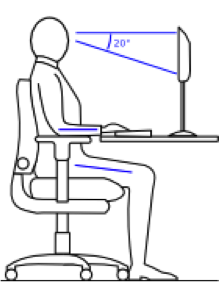
\includegraphics[width=0.8\textwidth,height=0.5\textheight,keepaspectratio]{imgs/health-safety-5.png}
\end{center}
\end{column}
\begin{column}{0.33\textwidth}
\begin{center}

\includegraphics[width=0.8\textwidth,height=0.5\textheight,keepaspectratio]{imgs/health-safety-3.png}\\

\includegraphics[width=0.8\textwidth,height=0.5\textheight,keepaspectratio]{imgs/health-safety-6.png}
\end{center}
\end{column}
\end{columns}
\end{frame}

\section{Who are we?}
\begin{frame}{UIS: Research and Institutional Services Division}
Your trainers for today will be:\\
\begin{itemize}
  \item Paul Sumption --- Research Computing Technical Liaison
    \item Mark Sharpley --- Computer Officer, WT/MRC Stem Cell Institute
  \item\alert{Please ask questions and let us know if you need assistance.}
\end{itemize}
\end{frame}

\section{More about your trainers}
\begin{frame}{Paul Sumption}
\begin{itemize}
  \item Advising users on Research Computing Services run by UIS
  \item Part of the Research Computing Team
  \item Experienced Linux sysadmin 
  \item Trainer for the introduction to HPC (High Performance Computing) course
  \item\alert{The HPC course is running tomorrow, raise your hand if you are on it!}
\end{itemize}
\end{frame}

\section{More about your trainers}
\begin{frame}{Mark Sharpley}
\begin{itemize}
  \item Computer Officer in the School of Biological Sciences
  \item Linux sysadmin 
  \item Building servers and run a small compute cluster 
\end{itemize}
\end{frame}

\section{Material Pt 1}
\begin{frame}{Introduction: Course Material}
\begin{itemize}
\item Today's course uses a modified version of material that was written for UIS MCS Linux
\item UIS MCS facilities: \url{https://help.uis.cam.ac.uk/service/devices-networks-printing/managed-desktops/mcs/mcr-rooms} 
\item Details of the MCS Linux service: \url{https://help.uis.cam.ac.uk/service/devices-networks-printing/managed-desktops/mcs/basiclinux} 
\end{itemize}
\end{frame}

\section{Material Pt 2}
\begin{frame}{Introduction: Material}
The course has been designed as 'self paced':
\begin{itemize}
\item a) Obtain an MCS account, download the course and then start teaching yourself using a MCS Linux PC and the notes
\item b) Book a place on a UIS course. There is an instructor present to help you if you get stuck on the exercises
\item Our course is being delivered at the Bioinformatics Training Facility
\item We have made quite a few changes to the original material
\item We have tested the exercises but please let us know if you find a mistake in the material 
\end{itemize}
\end{frame}

\section{Introduction: Other Linux Courses}
\begin{frame}{Other Courses}
\begin{itemize}
\item Unix: Introduction to the Command Line Interface (Self-paced)
\small {\url{https://www.training.cam.ac.uk/ucs/Course/ucs-unixintro1}} 
\item{The course that runs on MCS Linux}
\pause
\item Shell scripting:
\item Unix: Simple Shell Scripting for Scientists
\small {\url{https://www.training.cam.ac.uk/ucs/Course/ucs-scriptsci}} 
\end{itemize}
\end{frame}

\section{Introduction: Format for today}
\begin{frame}{Format for today}
\begin{itemize}
\item We have split the self paced material into several sections
\item Before each section we will present some slides to introduce the topic
\item You will then have time to attempt the self paced material for the section
\item During self paced work we will assist you, just put your hand up if you are stuck
\item Your instructors can demonstrate exercises as needed
\end{itemize}
\end{frame}

\section{Today's Session}
\begin{frame}{Today's Session}
\begin{itemize}
\item Course material will be displayed on the left and right hand side screen
\item The central screen will display the course notes or demonstrating exercises
\item Your PC will already be booted into Linux 
\end{itemize}
\end{frame}

\section{Usernames and Passwords}
\begin{frame}{Usernames and passwords}
\begin{itemize}
\item Your desktop PC has a local user account 
\item When we get to the remote server exercise we will give you each a username and password for the remote machine
\end{itemize}
\end{frame}

\section{Course Material}
\begin{frame}{Course Material}
\begin{itemize}
\item We will demonstrate how to access the Course Material on your PC
\item You will find a copy of the course material in your home folder
\item There is a PDF of course notes and exercises
\item The folder 'Linux Intro' contains files and folders needed for the exercises
\item There is a zip file 'LinuxIntro.tgz' which will be use during the remote server exercises 
\end{itemize}
\end{frame}

\section{File Management}
\begin{frame}{Files}
\begin{itemize}
\item Click this icon to start the file manager:

\includegraphics{imgs/files.png}
\item This is similar to Explorer on Windows or Finder on a Mac
\end{itemize}
\end{frame}

\section{Home Folder}
\begin{frame}{Home Folder}
\begin{itemize}
\item Click Files
\item A window will open and display your home folder
\item Click on the 'Linux Intro' folder
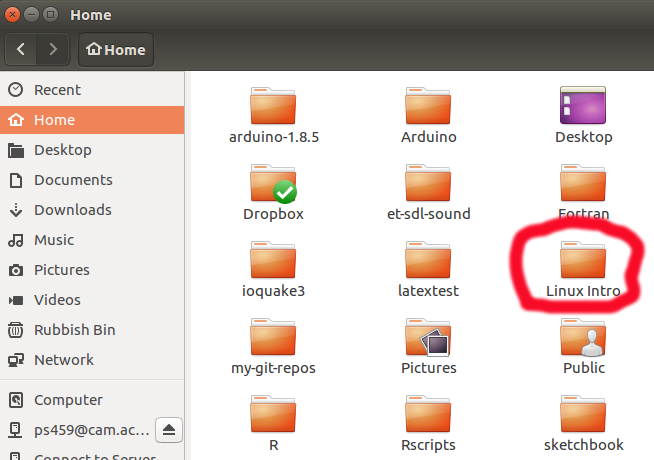
\includegraphics[height=0.5\textheight]{imgs/HomeFolder.png}
\end{itemize}
\end{frame}

\section{Course Folder}
\begin{frame}{Open the Course Folder}
\begin{itemize}
\item Click on the 'Beginners-linux-notes.pdf' folder
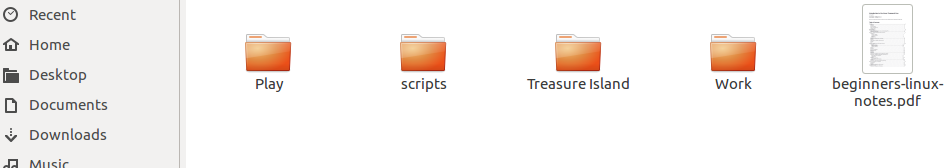
\includegraphics[height=0.2\textheight]{imgs/LinuxIntroFolder.png}
\end{itemize}
\end{frame}

\section{Your Desktop}
\begin{frame}{Your Desktop}
\begin{itemize}
\item Your desktop should look similar to this, notes open, home folder open
\item\alert{Raise your hand if you need help}
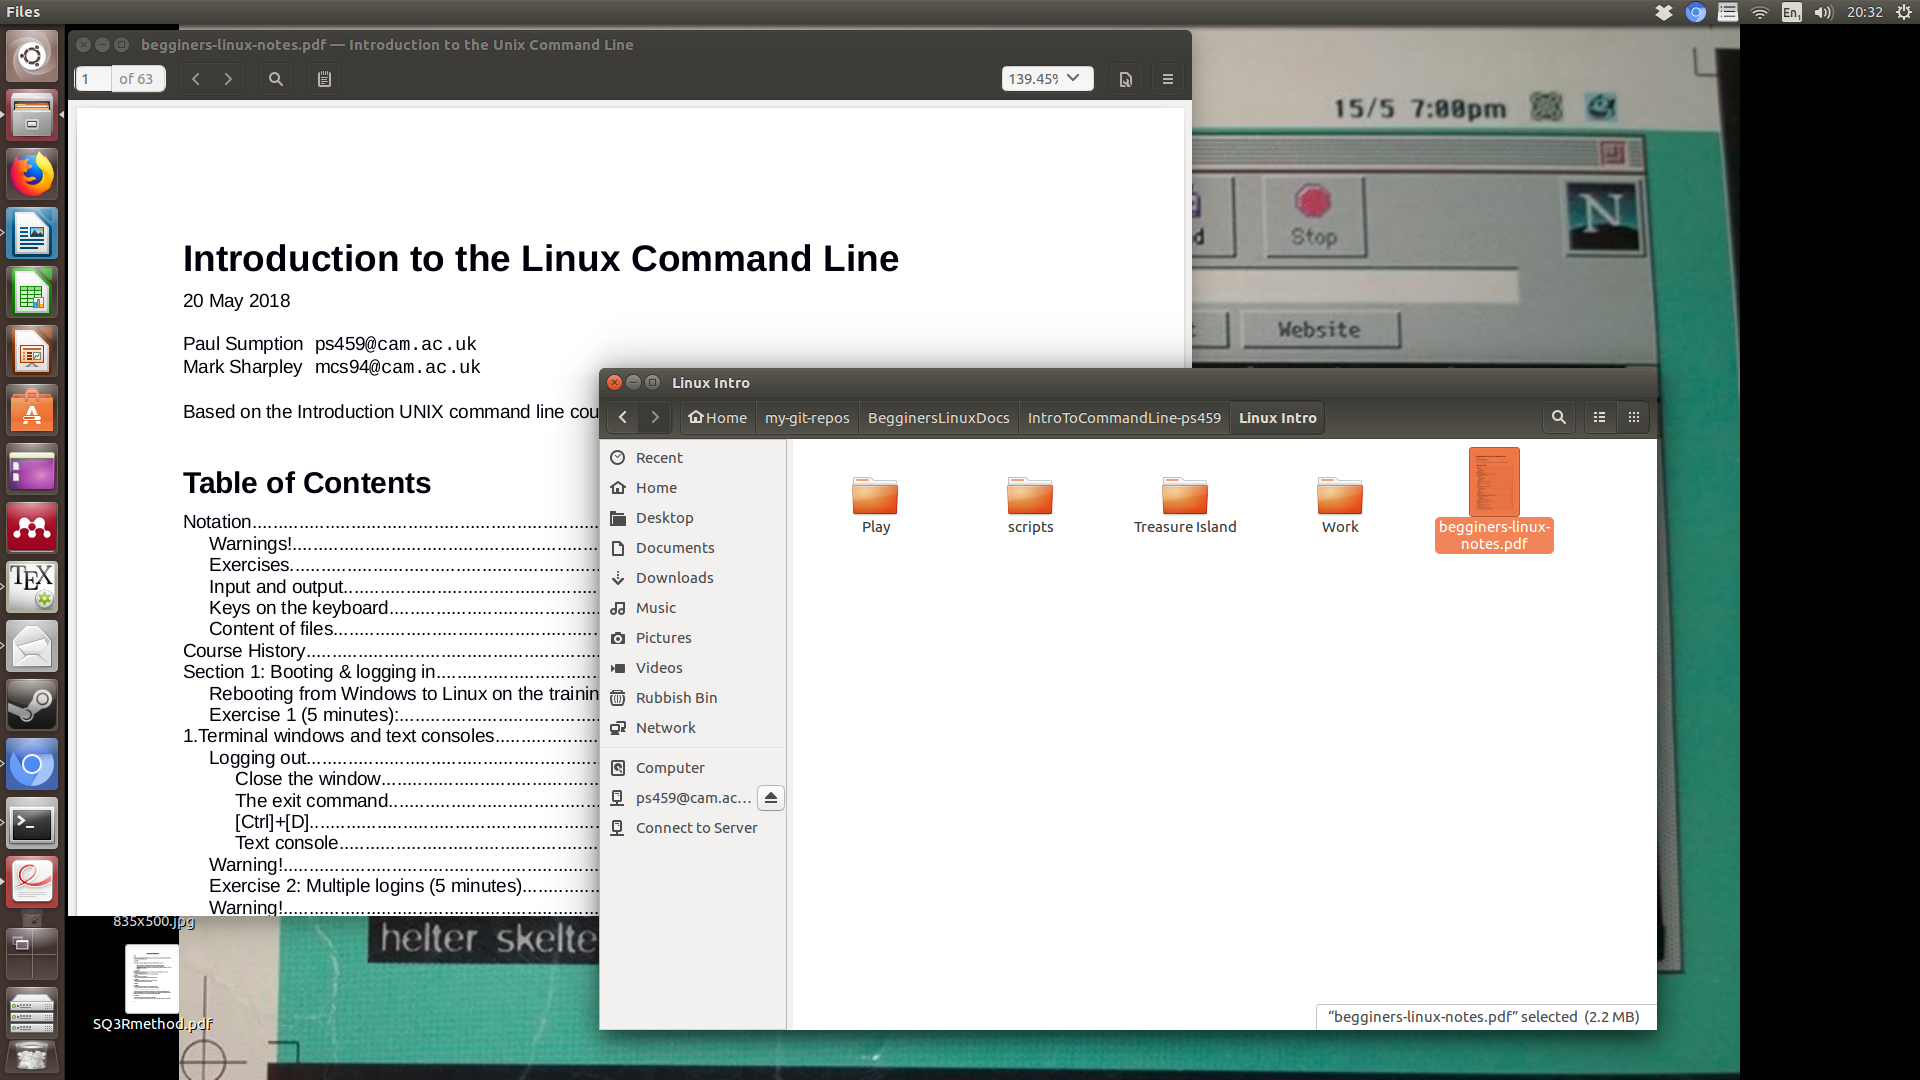
\includegraphics[height=0.5\textheight]{imgs/Desktop.png}
\end{itemize}
\end{frame}





\part{Terminals}
\begin{frame}
\partpage
\end{frame}

\section{Terminal windows}
\begin{frame}{Terminal windows}
\begin{itemize}
\item Most of our work will be using the Linux terminal
\item The icon you click to start the terminal looks like this:

\includegraphics{imgs/terminal-icon.png}
\item The bar on the left hand side is called your 'Launcher'
\end{itemize}
\end{frame}

\section{The Launcher}
\begin{frame}{Section 1: The Launcher}
\begin{itemize}
\item Only a few applications are in your launcher
\item You can search for more applications i.e. gedit
\item Use the icon in the top left corner:
\begin{figure}[h]
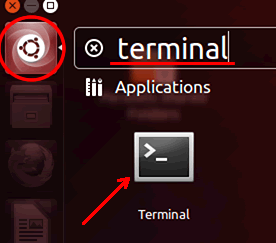
\includegraphics[height=0.3\textheight]{imgs/ubuntu-search-icon.png}
\end{figure}
\end{itemize}
\end{frame}

\section{Terminals on remote systems}
\begin{frame}{Section 1: Terminals on remote system}
\begin{itemize}
\item It is quite common to only have command line terminal access on a remote machine
\item I would assume most of you have Mac or Windows laptops
\item Mac users, OS X has a built in terminal
\item Windows users, you will need to install Putty to get a terminal client
\item We have put details about this in the notes
\end{itemize}
\end{frame}

\section{Text consoles}
\begin{frame}{Section 1: Text Consoles}
\begin{itemize}
\item Linux server administrators often dispense with the graphical environment entirely
\item One of the exercises involves starting a text based console
\item When you push the keys \begin{semiverbatim}[Ctrl]+[Alt]+[F2]\end{semiverbatim} your desktop will disappear!
\item It's not gone, you've just dropped down to a text based console
\item Remember that \begin{semiverbatim}[Ctrl]+[Alt]+[F7]\end{semiverbatim} returns you back to the graphical interface
\end{itemize}
\end{frame}

\section{Exercises}
\begin{frame}{Section 1: Exercises}
\begin{itemize}
\item In the notes go to Section 1: Terminal windows and text consoles
\item Read the notes for Section 1 
\item Attempt exercises 1 and 2
\item Raise your hand if you are stuck
\item We can demonstrate or explain an exercise
\end{itemize}
\end{frame}
\part{Navigating the file system}
\begin{frame}
\partpage
\end{frame}

\section{Navigating the file system in the CLI}
\begin{frame}{Section 2: The file system}
\begin{itemize}
\item This section teaches you how to navigate the file system using the command line
\item Using cd to move between directories
\item Using ls for listing directory contents
\item Quoting: How we handle directories and files with spaces in the name
\item Escaping: How to ignore special characters
\item Renaming and deleting files and directories
\end{itemize}
\end{frame}

\section{autocomplete}
\begin{frame}{Section 2: Tab autocomplete}
\begin{itemize}
\item If you start typing a filename, path or command and then hit tab...
\item Linux tries to autocomplete for you
\item This will save you time
\end{itemize}
\end{frame}

\section{Exercises}
\begin{frame}{Section 2: Navigating the File System}
\begin{itemize}
\item In the notes go to Section 2: Navigating the File System
\item Read the notes for Section 2
\item Attempt exercises 3 and 4
\item Raise your hand if you are stuck
\item We can demonstrate or explain an exercise
\end{itemize}
\end{frame}

\section{Command cheat sheet}
\begin{frame}{Section 2: Where am I?}
\begin{itemize}
\item As you move back and forth between directories...
\item Its easy to get lost
\item{\alert{\footnotesize cd \textless dirname \textgreater } - change into a directory }
\item{\alert{\footnotesize ls \textless dirname \textgreater } - list the contents of a directory}
\item{\alert{\footnotesize cd or cd \path{~}} - change into your home folder}
\item{\alert{\footnotesize cd .. } - change back one folder}
\item{\alert{\footnotesize pwd } - print working directory}
\end{itemize}
\end{frame}

\part{Section 3: Anatomy of a command}
\begin{frame}
\partpage
\end{frame}

\section{Commands}
\begin{frame}{Section 3: Commands}
\begin{itemize}
\item A command is an instruction given by a user telling a computer to do something
\item Commands often take options
\item Commands often take arguments
\item Options can be used in long form i.e. ls --all 
\item Options can be used in short form i.e ls -a
\end{itemize}
\end{frame}

\section{autocomplete}
\begin{frame}{Section 3: Getting help}
\begin{itemize}
\item Command line help is available as 'man' pages
\item This is short for manual
\item They can be quite detailed
\item Most commands can be used with the switch '--help'
\item As a beginner '--help' is probably easier
\end{itemize}
\end{frame}

\section{Exercises}
\begin{frame}{Section 3: Exercises}
\begin{itemize}
\item In the notes go to Section 3: Anatomy of a command
\item Read the notes for the section 
\item Attempt exercises 5 and 6
\item Raise your hand if you are stuck
\item We can demonstrate or explain an exercise
\end{itemize}
\end{frame}


\part{Section 4: Remote access to other Linux systems}
\begin{frame}
\partpage
\end{frame}

\section{Remote Access}
\begin{frame}{Section 4: Remote Linux systems}
\begin{itemize}
\item Most Linux systems allow remote log in
\item This is provided you have a user account on the remote machine
\item Most of the Linux systems you'll want to work with will be remote
\end{itemize}
\end{frame}

\section{Security}
\begin{frame}{Security}
\begin{enumerate}
\item{\alert{Keep your password (or private key passphrase) safe.}}
\pause
\item{\alert{Always choose strong passwords.}}
\pause
\item{\alert{Your UIS password is used for multiple systems so keep it secure!}}
\pause
\item{Keep the software on your laptops/tablets/PCs up to date this includes home computers especially if you are using the VPN to connect in.}
\pause
\item{Don't share accounts (this is against the rules anyway).}
\end{enumerate}
\end{frame}

\section{Remote Access Software}
\begin{frame}{Section 4: Remote Access Software}
\begin{itemize}
\item Remote access is provided by SSH
\item Files can be transferred by scp, sftp and rsync
\item There are other tools, we cover the ones that most systems have
\end{itemize}
\end{frame}

\section{Exercises}
\begin{frame}{Section 4: Exercises}
\begin{itemize}
\item In the notes go to Section 4: Remote Linux systems
\item {\textcolor{red}{We need to give you a username and password for the remote server}}
\item Read the notes for the section 
\item Attempt exercises 7 and 8
\item Raise your hand if you are stuck
\item We can demonstrate or explain an exercise
\end{itemize}
\end{frame}

\section{Command cheat sheet}
\begin{frame}{Section 2: Where am I?}
\begin{itemize}
\item At the back of your notes there is an SFTP cheat sheet
\end{itemize}
\end{frame}
\part{Launching graphical applications}
\begin{frame}
\partpage
\end{frame}

\section{Graphical Applications}
\begin{frame}{Section 5: Launching graphical applications}
\begin{itemize}
\item If your machine has X Windows you can launch graphical applications from the command line
\item The HPC course explains more about X Windows and X Window forwarding
\item X forwarding is an advanced topic, we will just give an overview
\end{itemize}
\end{frame}

\section{Exercises}
\begin{frame}{Section 5: Exercises}
\begin{itemize}
\item In the notes go to {Section 5: Launching graphical applications}
\item Read the notes for Section 5 
\item Attempt exercises 9 to 11
\item Raise your hand if you are stuck
\item We can demonstrate or explain an exercise
\end{itemize}
\end{frame}
\part{Section 6: Command line editing}
\begin{frame}
\partpage
\end{frame}

\section{Command Line Editing}
\begin{frame}{Section 6: Command line editing}
\begin{itemize}
\item Often you'll type a command or want to re-type a command
\item You can use keyboard shortcuts to find previously typed commands
\item The history and ctr + r are very useful
\end{itemize}
\end{frame}

\section{Finding Text}
\begin{frame}{Section 6: Grep}
\begin{itemize}
\item Often you'll want to search text files
\item grep is a powerful tool and can be used to find words or strings
\item Advanced users learn tools such as sed and awk to manipulate text
\item sed and awk are worth learning once you advance to shell scripting
\item sed -ie 's/annote/note/g' Dissertation-2-script.bib
\item Changes the word annote to note....
\end{itemize}
\end{frame}

\section{The Date}
\begin{frame}{Section 6: The Date}
\begin{itemize}
\item The date command lets you manipulate the format of the date
\item It becomes useful when you start writing scripts
\end{itemize}
\end{frame}

\section{The date in a script}
\begin{frame}{Section 6: The Date in a script}
\begin{figure}[h]
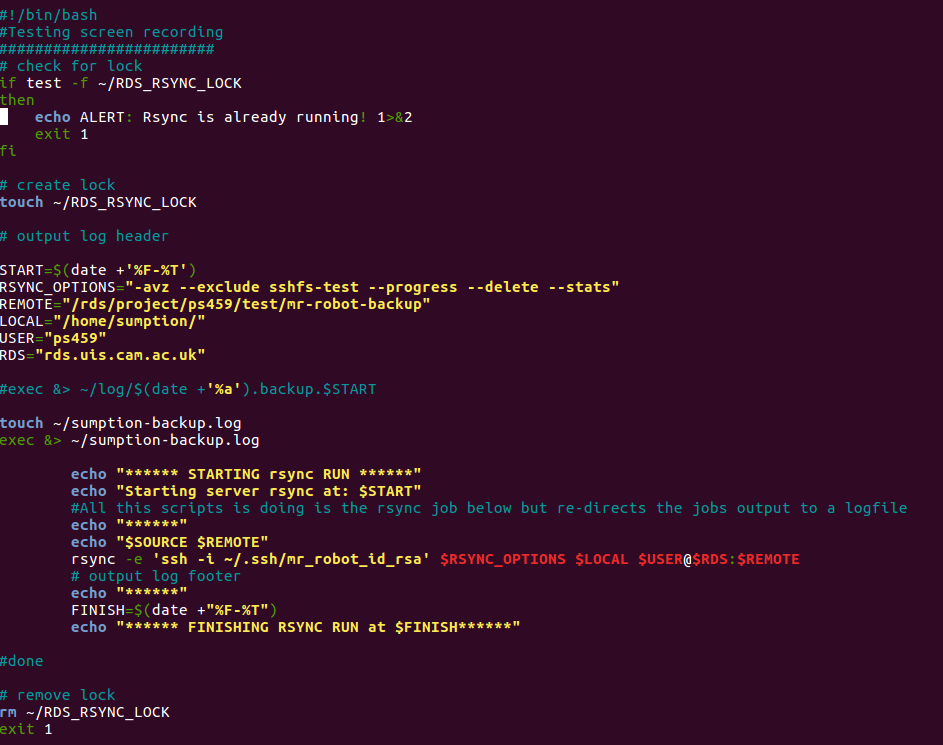
\includegraphics[height=0.8\textheight]{imgs/script-date.png}
\end{figure}
\end{frame}

\section{Exercises}
\begin{frame}{Section 6: Exercises}
\begin{itemize}
\item In the notes go to {Section 6: Command line editing}
\item Read the notes for the section 
\item Attempt exercises 14 to 16
\item Raise your hand if you are stuck
\item We can demonstrate or explain an exercise
\end{itemize}
\end{frame}


\part{Redirecting data and piping commands}
\begin{frame}
\partpage
\end{frame}

\section{Command Line Editing}
\begin{frame}{Section 7: Redirecting data and piping commands}
\begin{itemize}
\item Often you will want to send the output of one command into another
\item Maybe you want to combine multiple files
\item Combining pipes and the cat command is a good way to do this
\end{itemize}
\end{frame}


\section{Exercises}
\begin{frame}{Section 7: Exercises}
\begin{itemize}
\item In the notes go to {Section 7: Redirecting data and piping commands}
\item Read the notes for Section 7 
\item Attempt exercises 17 to 19
\item Raise your hand if you are stuck
\item We can demonstrate or explain an exercise
\end{itemize}
\end{frame}


\part{File name wild cards}
\begin{frame}
\partpage
\end{frame}

\section{Wild Cards}
\begin{frame}{Section 8: File name wild cards}
\begin{itemize}
\item Sometimes you may wish to find a file or folder without knowing the full name
\item Wild cards can help you do this
\item Your are substituting parts of the name
\item Different operators have different meanings
\item Useful when working with lots of similarly named files i.e. from HPC or Biology software
\end{itemize}
\end{frame}


\section{Exercises}
\begin{frame}{Section 8: Exercises}
\begin{itemize}
\item In the notes go to {Section 8: File name wild cards}
\item Read the notes for Section 8 
\item Attempt exercises 20
\item Raise your hand if you are stuck
\item We can demonstrate or explain an exercise
\end{itemize}
\end{frame}


\part{Environment variables}
\begin{frame}
\partpage
\end{frame}

\section{Environment variables}
\begin{frame}{Section 9: Environment variables}
\begin{itemize}
\item Sometimes you will need to manipulate your PATH
\item A good example is when you install software inside your home folder
\item We will manipulate the PATH in the next section on shell scripting
\end{itemize}
\end{frame}


\section{Exercises}
\begin{frame}{Section 9: Environment variables: Exercises}
\begin{itemize}
\item In the notes go to {Section 9: Environment variables}
\item Read the notes for Section 9
\item There are no exercises for this section
\item It is important to understand what PATH does as we will manipulate it in the next section
\end{itemize}
\end{frame}


\part{Shell Scripting}
\begin{frame}
\partpage
\end{frame}

\section{Section 10: Trivial shell scripts}
\begin{frame}{What are shell scripts?}
\begin{itemize}
\item An advantage of the command line is that we can run a "script" of commands
\item The script can then be kept for later reuse or given to other people for them to use
\item Scripting is useful when we have long repeatable tasks
\end{itemize}
\end{frame}

\section{Exercises}
\begin{frame}{Section 10: Exercises}
\begin{itemize}
\item In the notes go to {Section 10: Trivial shell scripts}
\item Take time to read the notes, this is a harder section 
\item Attempt exercises 21 to 24
\item Raise your hand if you are stuck
\item We can demonstrate or explain an exercise
\end{itemize}
\end{frame}


\part{Closing Session}
\begin{frame}
\partpage
\end{frame}

\section{4pm: Closing Session}
\begin{frame}{Closing Session}
\begin{itemize}
\item Hopefully you have completed most of the exercises
\item Please complete the online feedback form
\item Between 4pm and 4.30pm we will take questions
\item Please speak to us and give feedback
\item We will then start to pack up and leave by 5pm
\end{itemize}
\end{frame}

\section{4.30pm Close}
\begin{frame}{Closing Session}
\begin{itemize}
\item Thanks for attending!
\item Well done on starting to learn Linux
\end{itemize}
\end{frame}



\end{document}
